%%%%%%%%%%%%%%%%%%%%%%%%%%%%%%%%%%%%%%%%%%%%%%%%%%%%%%%%%%%%%%%%%%%%%%%%%%%%%%%%
%%                           ONDER DE LOEP ARTIKEL                            %%
%%%%%%%%%%%%%%%%%%%%%%%%%%%%%%%%%%%%%%%%%%%%%%%%%%%%%%%%%%%%%%%%%%%%%%%%%%%%%%%%

\artikelfoto{Parameterkrommen}{}{Michel Roelens \\ Luc Van den Broeck}{img/clothoidebanner.jpg}

\startcontents[inhoudloep]	% om inhoud voor het loep artikel te beginnen

\begin{multicols}{2}
	
	\inhoudstafelloep			% om inhoudstafel voor het loep artikel te tonen
	
	%% Gebruik \section{titel} en \subsection{titel} om genummerde tussentitels te maken
	\section{Inleiding}
	
	Parameterkrommen vormen geen expliciet onderwerp in de leerplannen wiskunde. Ze komen als toepassing in onze lessen en handboeken terug, bijvoorbeeld bij de goniometrische cirkel die doorlopen wordt in functie van de middelpuntshoek $\alpha$. Occasioneel ook maken we een oefening op raaklijnen aan parameterkrommen of op oppervlakten van een gebied ingesloten door een parameterkromme. 
	
	In \emph{paragraaf 2} leiden we het begrip parameterkromme in en bekijken we de mogelijkheden om een grafiek te maken met GeoGebra.
	
	In de fysica zijn parametervergelijkingen aantrekkelijke werktuigen om een beweging te beschrijven in functie van de tijd. Voor de schuine worp van een puntmassa bijvoorbeeld kunnen we de positie op de $x$-as en op de $y$-as afzonderlijk  beschrijven in functie van de tijd. In \emph{paragraaf 3} belichten we onder andere het verband tussen parameterkrommen in de fysica en de snelheidsvectoren die raken aan de baan van een bewegend voorwerp.
	
	Vaak kan een kromme zowel beschreven worden door een vergelijking in de cartesiaanse coördinaten $x$ en $y$ als door een parametervergelijking in $x$, $y$ en $t$. Bij de gewone vergelijking in $x$ en $y$ is het makkelijk om na te gaan of een punt met gegeven coördinaten op de kromme ligt. Ook symmetrieën rond de $x$-as, de $y$-as en de oorsprong zijn eenvoudig te detecteren. Bij parameterkrommen komt er een aspect bij. We zien hoe de baan doorlopen wordt: in welke zin, met welk beginpunt en met welke snelheid. Hier is de vraag of een punt met gegeven coördinaten op de kromme ligt, moeilijker op te lossen. 
	
	In \emph{paragraaf 4} geven we een voorbeeld van een baan die niet zo makkelijk met een vergelijking in de cartesiaanse coördinaten $x$ en $y$ is uit te drukken. We stellen de parametervergelijkingen op van een baan in de vorm van een ei, het ei van Fritz Hügelschäffer.
	
	Het historisch belang van bepaalde parameterkrommen wordt onderzocht in \emph{paragraaf 5}. In de tweede eeuw voor onze jaarrekening werd aangetoond dat de cissoïde (of de klimopkromme) van Diocles gebruikt kan worden als hulpmiddel voor de verdubbeling van de kubus. De ribbe  van een kubus vinden die de dubbele inhoud heeft van een kubus met een gegeven ribbe, is onmogelijk met het klassieke Griekse gereedschap: een passer en een liniaal. Dat werd pas twee millennia na Diocles bewezen.
	
	In de zeventiende eeuw werd een andere parameterkromme populair: de cycloïde. Ze werd geïntroduceerd als de baan van een punt op de rand van een schijf die zonder slippen over een rechte rail rolt. Later werd deze kromme in verband gebracht met de snelste glijbaan van een punt $A$ naar een punt $B$ en werd ze ingezet om slingerklokken een vaste periode te geven wanneer hun slingeruitwijking verstoord werd, bijvoorbeeld op zee. 
	
	Historische opdrachten zoals die van de cycloïde en de cissoïde kunnen de leerlingen helpen om in te zien welke weg de meetkunde in het verleden heeft afgelegd, van de studie van de meetkundige eigenschappen van bepaalde krommen door middel van axioma's en stellingen (de synthetische meetkunde) naar beschrijvend met vergelijkingen en coördinaten (de analytische meetkunde). Een rode draad in deze evolutie is de onmogelijkheid om bepaalde problemen op te lossen met een beperkte gereedschapskist aan hulpmiddelen. 
	
    In \emph{paragraaf 6} gebruiken we moderne technieken om een parameterkromme te tekenen waarvan (de $x$- en de $y$-coördinaat van) de punten zelfs niet exact te berekenen zijn. Het thema van deze paragraaf is de `clothoïde'. Deze kromme heeft toepassingen in de wegenbouw. 
    
    Het niet exact berekenbaar zijn van waarden is een klassiek probleem in de wiskunde. Denk maar aan de nulpunten van bepaalde functies, die enkel benaderd kunnen worden door iteratieve technieken. Omdat de computationele vaardigheden aan belang winnen, laten we onze leerlingen een programma schrijven om de punten van een clothoïde benaderend te plotten. We zien deze toepassing eerder als een project voor de vrije ruimte wiskunde in het vijfde en het zesde jaar.
	
	\section{Verbind de stippen van 1 tot 100}
	
Iedereen heeft een tekenpuzzel met zulke opdracht wel eens gemaakt: ``Verbind de stippen van 1 tot 100 met een vloeiende lijn en kijk wie je toelacht''. Meestal kun je aan de bijgetekende oogjes en aan de attributen meteen zien dat het eindresultaat een Calimero of een Minnie Mouse moet zijn. Na het verbinden ontstaat er een kleurplaat, waarop kinderen, en soms ook volwassenen, zich duchtig kunnen uitleven.

Als ik zulke opgave aan mijn leerlingen voorschotel, kan ik niet aan een wiskundige notatie weerstaan. Een opgave met 13 genummerde punten in het vlak zou ik noteren als een functie van de verzameling $\{0, 1, 2, \dots, 11, 12 \}$ naar $\R^2$, bijvoorbeeld:

\[f: \{0, 1, 2, \dots, 11, 12 \} \to  \R^2: \]
\[t \mapsto \left(\cos(t)-3 \cos \left(\frac{t}{2} \right),-\sin(t) \right).\]

De opgave klinkt heel wat wiskundiger met deze functienotatie.

\afbeelding{img/viske1.jpg}{Verbind de punten van 0 tot 12.}{fig:stippen}

Wat me als kind bij deze opgaven stoorde, was dat al mijn vriendjes een andere vis tekenden die bij deze stippen hoorde. Sommige vriendjes verbonden de opeenvolgende punten met een liniaal. Ik niet. Ik vond het leuk om wat extra krullen en fantasietjes in de oplossing te verwerken, zoals in \autoref{fig:verbondenstippen}. Volgens mij was dit ook een juiste oplossing. 

\afbeelding{img/viske2.jpg}{Zo kan het ook.}{fig:verbondenstippen}

Een techniek om minder variatie te krijgen in de oplossingen, bestaat er mogelijk in het aantal punten te verhogen. Zo zou je de opgave kunnen veranderen in de onderstaande, zonder afbreuk te doen aan de voorgaande gegevens.

\[f: \left\{ 0, \frac{1}{2}, 1, \frac{3}{2}, \dots, 11,  \frac{23}{2}, 12, \frac{25}{2}  \right\} \to  \R^2: \]
\[t \mapsto \left(\cos(t)-3 \cos \left(\frac{t}{2} \right),-\sin(t) \right)\]

\afbeelding{img/viske3.jpg}{Verbind de 26 punten.}{fig:viskedrie}

Ondanks het kwantitatieve verschil in het aantal gegevens, blijft het probleem nog steeds bestaan. Wie van slechte wil is, kan een kroontje op het hoofd van de vis tekenen en kan hem een baard aanmeten. 

Het aantal punten nog een aantal keer verhogen, helpt ogenschijnlijk wel om alle pixels van de kromme op het scherm geplot te krijgen. Maar wiskundig is dit niet voldoende. Als een wiskundige door een vergrootglas kijkt, ziet hij nog steeds gaten tussen de voorgedrukte punten. Er is slechts één manier om een eenduidige tekening te krijgen. Het domein van de functie moet een interval zijn. De opgave kunnen we bijvoorbeeld omvormen tot:

\[f: [0, 4 \pi] \to  \R^2: \]
\[t \mapsto \left(\cos(t)-3 \cos \left(\frac{t}{2} \right),-\sin(t) \right).\]


\afbeelding{img/viske4.jpg}{Een afbeelding van een interval naar het vlak}{fig:viske4}


Als puzzelopgave voor kinderen uit de lagere school is deze opdracht nu waardeloos geworden. De opgave is immers gelijk aan de oplossing. Maar als intro voor een les van parameterfuncties kan ze wel dienen. Een parameterfunctie is een functie van een interval naar het vlak $\R^2$ of naar de driedimensionale ruimte $\R^3$. De grafiek van een parameterfunctie is een vlakke of een ruimtelijke kromme. Ze hoeft niet gesloten te zijn.

\subsection{Meerdere parametriseringen}

Het visje hierboven is cyclisch geparametriseerd. Als je de coördinaten van het punt waarvoor $t=0$ berekent, merk je dat  je in het midden van de staart zit. Als je $t$ laat aangroeien, duik je eerst naar het onderste puntje van de staart en wandel je vervolgens in wijzerzin rond het vissenlichaam. Bij $t=2\pi$ bereik je het neusje van de zalm. Je wandelt vervolgens langs onder verder en bij $t=4\pi$ ben je weer bij de sta(a)rt. Als je de parameter $t$  nog verder laat oplopen, wandel je weer in je eigen voetsporen verder, cyclisch en met een periode van $4\pi$.

Hoewel de kromme die het visje beschrijft, eenduidig vast ligt, is de parametervoorstelling niet eenduidig. Stel dat je de grafiek tekent van de parameterfunctie:

\[f: [0, 4 \pi] \to  \R^2: \]
\[s \mapsto \left(\cos(s+2\pi )-3 \cos \left(\frac{s+2\pi}{2} \right),-\sin(s+2\pi) \right)\]

dan krijg je dezelfde vis. Bij $s=0$ zit je bij de neus, daarna loop je in dezelfde zin verder als voorheen en bij $s=2\pi$ zit je halverwege de staart. 

De viskromme is nu geherparametriseerd. In elk punt van de kromme is het verband tussen de parameters $s$ en $t$ gelijk: $t=s+2\pi$. Er bestaan ook herparametriseringen die de omloopzin van de kromme omkeren, bijvoorbeeld: $t=-s$. En je kunt er ook voor zorgen dat de kromme veel vlugger doorlopen wordt, bijvoorbeeld via de herparametrisering $s=10 \cdot t$.

\subsection{Een grafiek in GeoGebra}

GeoGebra is een van de populairste wiskundeprogramma's in het onderwijs. De software is gebruiksvriendelijk en gratis. De laatste jaren heeft dit programma een grote vooruitgang gemaakt op gebied van de plotinstructies. Parameterkrommen worden feilloos getekend. En ook impliciete krommen zien er zeer behoorlijk uit. Nochtans bijten vele andere wiskundepakketten hier de tanden op stuk.

Om in GeoGebra een parameterkromme in het vlak te tekenen, gebruik je de instructie: 
\[a=\textrm{Kromme } (x(t),y(t), t,\textrm{ begin}, \textrm{ eind}). \]

Voor een parameterkromme in de driedimensionale ruimte, vermeld je na het voorschrift voor de $y$-coördinaat ook nog het voorschrift voor de $z$-coördinaat.

In \autoref{fig:geogebrakromme} zie je de grafiek van de functie:
\[ \begin{cases}
x(t)= \cos(2t)+\frac{\cos(6t)}{3}+\frac{\sin(5t)}{5} \\
y(t)= \sin(2t)+\frac{\sin(6t)}{3}+\frac{\cos(5t)}{5}. 
\end{cases}\]

\afbeelding{img/geogebrakromme.jpg}{Een parameterkromme in GeoGebra}{fig:geogebrakromme}

Om een punt $A$ toe te voegen dat bijvoorbeeld parameterwaarde $t=0$ heeft, volstaat het dit punt te definiëren als $A=a(0).$

De rekenkracht van GeoGeobra laat ook toe om kunstige krommen met een dicht lijnenpatroon en een groot parameterbereik te tekenen. Zo zie je in \autoref{fig:geogebrakromme2} de grafiek van de parameterkromme
\[ \begin{cases}
x(t)= \sin(2,99t)\cdot \cos(\cos(8t)) \\
y(t)= \cos(2,99t)\cdot \sin(\sin(8t))
\end{cases}\]
voor de parameterwaarden $t \in [-16,16]$.

\afbeelding{img/geogebrakromme2.jpg}{Een artistieke parameterkromme}{fig:geogebrakromme2}

Een folietje is dat GeoGebra bij het tekenen van een gesloten parameterkromme het onderscheid kan aanvoelen tussen binnen en buiten. Als je kriskras over het vlak met een parameterkromme wandelt en je dwarst de kromme dan ga je van binnen naar buiten of van buiten naar binnen. Het binnengebied en het buitengebied kunnen apart ingekleurd worden waardoor ook weer kunstige plaatjes kunnen ontstaan. 

In \autoref{fig:binnenbuiten} worden binnen- en buitengebieden van de kromme:
\[ \begin{cases}
x(t)= \cos(t)+\frac{\cos(6t)}{2}+\frac{\sin(14t)}{3} \\
y(t)= \sin(t)+\frac{\sin(6t)}{2}+\frac{\cos(14t)}{3} 
\end{cases}\]
voor de parameterwaarden $t \in [0,2 \pi]$ op een andere manier gearceerd.

Het inkleuren met verschillende opvulpatronen vind je bij de instellingen van de grafiek: stijl | vulling of stijl | omgekeerde vulling.

\afbeelding{img/binnenbuiten.jpg}{Binnen- en buitenkant}{fig:binnenbuiten}

Misschien herken je deze kromme? Het is er eentje waarvan de coëfficiënten in het voorschrift niet doen vermoeden dat er een vijfvoudige rotatiesymmetrie is. Hoe je de vijfvoudige symmetrie kunt aantonen zonder een grafiek te maken, lees je in het Spinnenweb van UW38/1.

\section{Een bewegend punt in het vlak}

In de vorige paragraaf kwam al aan bod dat je een zelfde kromme op verschillende manieren kunt doorlopen. Je kunt in een ander punt starten, je kunt sneller of trager gaan, in de andere draaizin... De parameter wordt hierbij geïnterpreteerd als de tijd en de kromme is de baan die een bewegend punt volgt.

In deze paragraaf willen we kort ingaan op de `snelheid' waarmee het punt de kromme doorloopt.

\subsection{Snelheidsvector}

Je schopt een bal schuin naar boven. De plaats van de bal op elk tijdstip $t$ wordt beschreven door

$$\left\{ 
    \begin{array}{l}
         x(t) = 8t\\
         y(t) = 12t-5 t^2
    \end{array}
    \right.$$

met $t$ in seconden en $x$ en $y$ in meter.

In het vervolg van deze paragraaf laten we de eenheden m, s, $\frac{\mathrm{m}}{\mathrm{s}}$... weg in de berekeningen (niet doorvertellen aan de fysicacollega's).

Laten we deze parametervergelijkingen even interpreteren. De bal wordt bekeken als een punt. Voor $t=0$ is de bal in het punt $(0, 0)$. De bal vertrekt op de grond. De $x$-coördinaat neemt met een vaste snelheid toe. De wrijving met de lucht wordt hierbij verwaarloosd. De $y$-coördinaat neemt eerst toe, dan af. Die coëfficiënt $5$ is een afronding van $\frac{1}{2}g$, met $g=9,81$, de vertraging door de zwaartekracht (in $\frac{\mathrm{m}}{\mathrm{s^2}}$), die de bal recht naar beneden trekt. Het domein voor de parameter $t$ is beperkt tot de waarden waarbij $y\ge0$:  de parabolische baan van de bal begint en eindigt op de grond. Dus $t\in [0; 2,4]$. 

We kunnen de baan in GeoGebra tekenen met de instructie:

$$a=\text{Kromme}(8t,12t-5t^2,t,0,2.4).$$

Om de bal te zien bewegen, kunnen we een punt op de kromme plaatsen en dit punt `animeren'. Je kunt de bal een spoor laten maken. Door de `animatiesnelheid' te verhogen, kun je zorgen voor een spoor van losse punten, met gelijke tussentijden. Bovenaan, in de buurt van de top, zijn die punten dichter bij elkaar dan opzij. Dit betekent dat de bal bovenaan trager gaat. De horizontale snelheid is overal gelijk: dit zie je aan het feit dat de punten van het spoor op gelijke horizontale afstanden van elkaar staan.

\afbeelding {img/Lbal1.png}{De baan van de bal}{fig:bal1}

Als we $t$ elimineren door $t$ in de tweede vergelijking te vervangen door $\frac{x}{8}$, krijgen we de cartesiaanse vergelijking van de parabolische baan:

$$y=\frac{3}{2}x-\frac{5}{64}x^2.$$ 

De cartesiaanse vergelijking beschrijft de kromme maar niet meer hoe de bal die doorloopt, op welk moment de bal waar is, hoe snel de bal beweegt... Deze informatie is verloren gegaan door het elimineren van de tijd $t$.

De snelheid waarmee de $x$-coördinaat van de bal verandert, is

$$\frac{\mathrm{d}x}{\mathrm{d}t}=8.$$ 

Die is constant. De snelheid waarmee de $y$-coördinaat verandert, is

$$\frac{\mathrm{d}y}{\mathrm{d}t}=12-10t.$$ 

Die is $12$ bij vertrek, en neemt per seconde af met $10$. Bv. $1$ seconde nadat de bal werd weggeschopt (dat is wanneer de bal in het punt $(8, 7)$ zit) is deze verticale snelheid nog maar $2$.

De snelheden waarmee de coördinaten veranderen, kunnen we bundelen tot een \emph{snelheidsvector}.

 $$
\begin{array}{cl}
    
     \overrightarrow{v}(t)& =\left(\dfrac{\mathrm{d}x}{\mathrm{d}t}, \dfrac{\mathrm{d}y}{\mathrm{d}t}\right) \\
     & =(8, 12-10t).
    
\end{array}
 $$


Deze snelheidsvector hangt af van $t$. Na $1$ seconde is het de vector $\overrightarrow{v}(1)=(8, 2)$; $8$ eenheden naar rechts en $2$ naar boven.

Merk op dat de snelheid van een bewegend punt in het vlak (of in de ruimte) altijd een vector is. De snelheden waarmee de coördinaten van het punt veranderen, worden de \emph{horizontale component} en de  \emph{verticale component} van de snelheid(svector) genoemd. De lengte van de snelheidsvector geeft de grootte van de snelheid weer ($v$ zonder pijltje):

$$
\begin{array}{cl}
     v(t)& =\sqrt{\left(\dfrac{\mathrm{d}x}{\mathrm{d}t}\right)^2+\left(\dfrac{\mathrm{d}y}{\mathrm{d}t}\right)^2} \\
     & = \sqrt{8^2+(12-10t)^2}\\
     & =2\sqrt{52-60t+25t^2}
\end{array}
$$

Hiermee kun je narekenen dat de grootte van de snelheid inderdaad minimaal is wanneer de bal het hoogst is, bij $t=\frac{6}{5}$, dus na $1,2$ seconden.

Als we bij de weggeschopte bal de snelheidsvector tekenen, aangrijpend in het punt waar de bal is, dan zie je dat die mooi raakt aan de parabool. De richting van de snelheidsvector is die van de raaklijn. 

\afbeelding{img/Lbal2.png}{Met snelheidsvectoren}{fig:bal2}

De richtingscoëfficiënt van de raaklijn in een punt met parameterwaarde $t$ is 

$$
\begin{array}{rl}
     \dfrac{\;\mathrm{d}y\;}{\mathrm{d}x}& \stackrel{\star}{=}\dfrac{\frac{\mathrm{d}y}{\mathrm{d}t}}{\frac{\mathrm{d}x}{\mathrm{d}t}}
     \vspace{1.5mm}\\
     & =\dfrac{12-10t}{8}
     \vspace{1mm}\\
     & =\dfrac{6-5t}{4}
\end{array}
$$

De gelijkheid $\star$ volgt uit de kettingregel

$$\frac{\mathrm{d}y}{\mathrm{d}x}\cdot \frac{\mathrm{d}x}{\mathrm{d}t}= \frac{\mathrm{d}y}{\mathrm{d}t}.$$

Laten we dit weer toepassen op één ogenblik: 1 seconde na het wegschoppen van de bal. We weten al dat de bal dan in het punt $(8, 7)$ zit en dat de snelheidsvector $(8, 2)$ is. De richtingscoëfficiënt van de raaklijn is bijgevolg $\frac{1}{4}$ en de vergelijking van de raaklijn in dat punt van de baan is $y-7=\frac{1}{4}(x-8)$, of nog

$$y=\frac{1}{4}x+5.$$

\subsection{Lissajousfiguren}

In de vorige opgave ontstaat de parabolische baan van de bal door combinatie van een eerstegraadsfunctie en een tweedegraadsfunctie: de $x$-coördinaat is een eerstegraadsfunctie van de tijd en de $y$-coördinaat een tweedegraadsfunctie van de tijd. De Franse natuurkundige Jules Antoine Lissajous (19de eeuw) bestudeerde combinaties van twee sinusfuncties, één voor de $x$-coördinaat en één voor de $y$-coördinaat. In de fysica spreekt men hierbij van de combinatie van twee \emph{harmonische trillingen} in twee richtingen loodrecht op elkaar. Dit had toepassingen bij de studie van radiogolven. Wij kunnen dergelijke \emph{Lissajousfiguren} vlot tekenen met GeoGebra; in de tijd van Lissajous was dat een hele klus met stemvorken en spiegels enz.

Leerlingen kunnen een GeoGebrafiguur maken voor de Lissajousfiguren bepaald door de volgende parametervergelijkingen met parameters $a, b, c$:

$$\left\{ 
    \begin{array}{l}
         x = \sin{at}\\
         y = \sin{(bt+c)}
    \end{array}
    \right.$$

Ze kunnen schuifknoppen maken voor de parameters $a, b$ en $c$. Ze krijgen de opdracht om mooie figuren maken, om zelf relevante vragen te stellen en die indien mogelijk te beantwoorden. We beperken ons in de lesactiviteit hieronder tot enkele voorbeelden.

\end{multicols}

\begin{lesactiviteit}{Enkele Lissajousfiguren}

\begin{multicols}{2}

\afbeelding[6,5cm]{img/Lliss1.png}{}{fig:Lliss1}

\afbeelding[6,5cm]{img/Lliss2.png}{}{fig:Lliss2}

\end{multicols}

\begin{multicols}{2}

\afbeelding[6,5cm]{img/Lliss4.png}{}{fig:Lliss4}

\afbeelding[6,5cm]{img/Lliss3.png}{}{fig:Lliss3}

\end{multicols}


    Bekijk de eerste Lissajousfiguur ($a=2, b=1, c=2$). De parametervoorstelling is
    
    $$\left\{ 
    \begin{array}{l}
         x = \sin{2t}\\
         y = \sin{(t+2)}
    \end{array}
    \right.$$
    
    \begin{vraagenantwoord}
    
    \item Waar begint de beweging bij $t=0$? Hoe gaat het punt verder als $t$ toeneemt? Voor welke $t$-waarde is de hele kromme doorlopen?
    
    \antwoord{Bij $t=0$ zit het punt in $(0, \sin 2)$. Dat is het bovenste snijpunt met de $y$-as. Als $t$ toeneemt, neemt $x$ toe; het punt gaat dus naar rechts. De periode van de horizontale beweging $x=\sin{2t}$ is $\pi$ en de periode van de verticale beweging $y=\sin{(t+2)}$ is $2\pi$. Hieruit volgt dat de periode van de gecombineerde beweging $2\pi$ is: na $2\pi$ zijn we rond en begint alles opnieuw.}
    
    \item Duid op de figuur de punten aan met parameterwaarden  $t=k\frac{\pi}{4}$ voor $k=0, 1 ...$ tot je weer bij dezelfde punten uitkomt.
    
    \antwoord{Dit zijn ze. De $x$-coördinaten komen mooi uit: $0, 1, 0, -1, 0, 1, 0, -1, 0$. De $y$-coördinaten komen niet mooi uit vanwege de term $2$ (radialen).}
    
    \afbeelding[5,5cm]{img/Lliss5.png}{}{fig:Lliss5}
    
    \item Voor welke $t$-waarden zit je in het punt waar de kromme zichzelf snijdt?
    
    \antwoord{We zien dat dit op de $x$-as gebeurt. De kromme snijden met de $x$-as geeft:}
    
    $$\sin(t+2)=0\Leftrightarrow t=k\pi-2\;\;(k\in\mathbb{Z})$$
    
    \emph{Voor $t\in[0,2\pi]$ zijn dit dus de parameterwaarden waar de kromme zichzelf snijdt: $t=\pi-2$ en $t=2\pi-2$}.
    
    \item Controleer met een afgeleide in welke punten de raaklijn verticaal is.
    
    \antwoord{We hebben:}
    
    $$
    \begin{array}{cl}
          \dfrac{\mathrm{d}x}{\mathrm{d}t}=0& \Leftrightarrow 2 \cos{2t}=0\\ 
          &\Leftrightarrow 2t=\frac{\pi}{2}+k\pi\;\;(k\in\mathbb{Z})\\
          &\Leftrightarrow t=\frac{\pi}{4}+k\frac{\pi}{2}\;\;(k\in\mathbb{Z})
    \end{array}
    $$
    
    \emph{De raaklijn is dus verticaal in de punten bij $t=\frac{\pi}{4}, \frac{3\pi}{4}, \frac{5\pi}{4}, \frac{7\pi}{4}$.}
    
    \end{vraagenantwoord}
    
    Bekijk nu de tweede Lissajousfiguur ($a=1, b=3, c=0)$). De parametervoorstelling is
    
    $$\left\{ 
    \begin{array}{l}
         x = \sin{t}\\
         y = \sin{3t}
    \end{array}
    \right.$$
    
    \begin{vraagenantwoord}[resume]
    
    \item Welke waarden moet $t$ aannemen om de hele kromme één keer te doorlopen? Beschrijf hoe het veranderlijk punt op de kromme beweegt.
    
    \antwoord{Als je begint bij $t=0$, dan start het punt in de oorsprong. Het volgt de kromme tot het punt $(1, -1)$. Dan is $t=\frac{\pi}{2}$. Dan keert het punt terug, langs de kromme, tot het punt $(-1,1)$. Op dat moment is $t=\frac{3\pi}{2}$. Dan keert het punt langs de kromme terug naar de oorsprong. Dan is $t=2\pi$ en zitten we terug in de beginpositie; als $t$ nog verder zou toenemen, zou alles zich herhalen.}
    
    \item De kromme lijkt verdacht op een stuk van de grafiek van een derdegraadsfunctie. Is dat echt het geval? Zo ja, bereken het voorschrift van deze derdegraadsfunctie, vanuit de parametervoorstelling.
    \newpage
    \antwoord{We hebben}
    $$
    \begin{array}{rl}
         y&= \sin{3t} \\
         & =\sin{(t+2t)}\\
         & =\sin{t}\cos{2t}+\cos{t}\sin{2t}\\
         & =\sin{t}\,(1-2\sin^2{t})+2\sin{t}\cos^2{t}\\
         & = \sin{t}\,(1-2\sin^2{t})+2\sin{t}\,(1-\sin^2{t})\\
         & = x(1-2x^2)+2x(1-x^2)\\
         & = -4x^3+3x
    \end{array}
    $$
    
    \emph{De kromme is het stuk van de grafiek van deze derdegraadsfunctie met $x,y\in [-1,1]$ .}
    
    \end{vraagenantwoord}
    
     Bekijk nu de derde Lissajousfiguur ($a=1, b=1, c=2$). De parametervoorstelling is
    
    $$\left\{ 
    \begin{array}{l}
         x = \sin{t}\\
         y = \sin{(t+2)}
    \end{array}
    \right.$$
    
    \begin{vraagenantwoord}[resume]
    
    \item Dit lijkt wel een ellips te zijn, met symmetrieassen die hoeken van $45^\circ$ maken met de coördinaatassen. Reken na of dit het geval is. 
    
    Een tip hierbij: als je het assenstelsel over $45^\circ$ in wijzerzin draait, ontstaan er nieuwe coördinaten $(X, Y)=\left(\frac{\sqrt{2}}{2} (x-y),\frac{\sqrt{2}}{2} (x+y)\right)$. Je moet dus nagaan of de kromme in dit nieuwe assenstelsel beschreven wordt door een canonieke ellipsvergelijking.
    
    \antwoord{We berekenen de $X$- en de $Y$-coördinaten uit van een punt van deze Lissajousfiguur:}
    
    $$ 
    \begin{array}{lll}
         X &= \frac{\sqrt{2}}{2} (x-y) & \\
         &= \frac{\sqrt{2}}{2} \left(\sin{t}-\sin{(t+2)}\right) & \\
         &=\sqrt{2} \cos{(t+1)}\sin{(-1)}&\text{(formule van Simpson)}\\
         Y&= \frac{\sqrt{2}}{2} (x+y) & \\
         &= \frac{\sqrt{2}}{2} \left(\sin{t}+\sin{(t+2)}\right) & \\
         &=\sqrt{2} \sin{(t+1)}\cos{1}&\text{(formule van Simpson)}\\
    \end{array}
    $$ 
    
    \emph{We elimineren $t$ door uit te drukken dat $\cos^2{(t+1)}+\sin^2{(t+1)}=1$. Hierbij merken we ook op dat $\sin^2{(-1)}=(-\sin{1})^2=\sin^2{1}$.}
    
    $$
    \cos^2{(t+1)}+\sin^2{(t+1)}=1\Leftrightarrow \frac{X^2}{2\sin^2{1}}+\frac{Y^2}{2\cos^2{1}}=1
    $$
    
    \emph{Dit stelt een ellips voor met halve grote as $\sqrt{2}\sin{1}\approx 1,19$ en halve kleine as $\sqrt{2}\cos{1}\approx 0,76$.}
    
    \end{vraagenantwoord}
        

    Bekijk ten slotte de vierde Lissajousfiguur ($a=4, b=3, c=0)$. De parametervoorstelling is
    
    $$\left\{ 
    \begin{array}{l}
         x = \sin{4t}\\
         y = \sin{3t}
    \end{array}
    \right.$$
    
    \begin{vraagenantwoord}[resume]
    
    \item Waar begint en eindigt de beweging, als je start bij $t=0$ en stopt wanneer de hele kromme getekend is? 
    
    \antwoord{Bij $t=0$ zitten we in de oorsprong. Als $t$ toeneemt, beweegt het punt naar rechtsboven. Omdat de periode van $x=\sin{4t}$ gelijk is aan $\frac{\pi}{2}$ en die van $y=\sin{3t}$ gelijk aan $\frac{2\pi}{3}$, zijn we bij $t=2\pi$ helemaal rond: vier periodes horizontaal en drie verticaal. Dit kun je controleren door met je vinger de kromme te volgen.}
    
    \item Oefen om deze kromme in één vlotte pennentrek te tekenen en kom dit aan bord demonstreren.
    
    \end{vraagenantwoord}
    

\end{lesactiviteit}


\begin{multicols}{2}


\section{Van cirkel naar ei}

    In de volgende lesactiviteit stellen de leerlingen parametervergelijkingen op van een `eikromme'. Er zijn verschillende wiskundige krommen die de vorm van een ei benaderen, de ene al wat getrouwer dan de andere. Het woord `eikromme' is dus niet de naam van een welbepaalde wiskundige kromme, zoals bv. dat het geval is met de naam `parabool'. De eikromme in de werktekst is die van de Duitser Fritz Hügelschäffer die hierover in 1948 zijn ei legde. Het voordeel is dat de constructie nauw aanleunt bij een klassieke constructie van een ellips.

    Voor leerlingen die al vertrouwd zijn met parametervoorstellingen van een cirkel en een ellips, is het begin herhaling.

 \end{multicols}
 

\begin{lesactiviteit}{Een ei ontwerpen}

In deze lesactiviteit starten we van een cirkel om er stap voor stap een (tweedimensionaal) ei van te maken. Telkens stel je hierbij parametervergelijkingen op.

Op een cirkel met middelpunt $O(0, 0)$ en straal $a$ nemen we een veranderlijk punt $P(x, y)$

    \afbeelding[6,2cm]{img/Lei1.png}{}{}
    
\begin{vraagenantwoord}

    \vraag{Druk $x$ en $y$ uit in functie van de middelpuntshoek $t$ (zie figuur). Anders gezegd, geef parametervergelijkingen van deze cirkel.}
    
    \antwoord{Dit geeft}
    $$\left\{ 
    \begin{array}{l}
         x = a \cos{t}\\
         y = a \sin{t}
    \end{array}
    \right.$$
    
\end{vraagenantwoord}

Om het gemakkelijk te maken, hebben we $P$ in het eerste kwadrant getekend, maar de parametervergelijkingen die je opschreef gelden ook voor $P$ in andere kwadranten. Als je $t$ laat variëren in $[0, 2\pi]$, dan doorloopt $P$ één keer de hele cirkel.

Nu willen we van een cirkel naar een ellips gaan. We vertrekken van de cirkel met middelpunt $O(0, 0)$ en straal $a$, en we platten die af door alle $y$-coördinaten te vermenigvuldigen met factor $\frac{b}{a}$. We veronderstellen dat $b<a$ zodat deze factor kleiner is dan $1$. Op die manier maken we een ellips met middelpunt $O$, grote as $2a$ en kleine as $2b$.

    \afbeelding[7,2cm]{img/Lei2.png}{}{}

\begin{vraagenantwoord}[resume]

    \vraag{Welke parametervergelijkingen levert dit op?}
    \antwoord{Dit geeft}
     $$\left\{ 
    \begin{array}{l}
         x = a \cos{t}\\
         y = b \sin{t}
    \end{array}
    \right.$$
    \vraag{Heeft de parameter $t$ nog steeds de betekenis van de middelpuntshoek horend bij punt $P$, dus de hoek tussen de positieve $x$-as en $[OP$?}
    \antwoord{Neen want $t$ is de middelpuntshoek horend bij het corresponderende punt $A$ van de grote cirkel. Bij het afplatten blijft het dezelfde waarde van $t$ in de parametervoorstelling, maar de middelpuntshoek verkleint (voor een punt in het eerste kwadrant).}
    
\end{vraagenantwoord}

Een mooie constructie van de punten van de ellips gaat als volgt: je tekent twee concentrische cirkels met middelpunt $O(0, 0)$, één met straal $a$ en één met straal $b$ ($b<a$). Beschouw een variabele middelpuntshoek $t$ en construeer een rechthoekig driehoekje $ABP$ zoals in de figuur. (Als $t$ een veelvoud is van $\frac{\pi}{2}$, klapt het driehoekje dicht.) Het punt $P$ beschrijft dan de ellips met grote as $2a$ en kleine as $2b$.
 
    \afbeelding[7,2cm]{img/Lei3.png}{}{}

\begin{vraagenantwoord} [resume]
    \vraag{Leg uit dat $P$ dezelfde ellips beschrijft als daarnet.}
    \antwoord{De $x$-coördinaat van $P$ is die van het punt $A$ van de grote cirkel dat bij $t$ hoort, dus $a \cos{t}$. De $y$-coördinaat van $P$ is die van het punt $B$ van de kleine cirkel dat bij $t$ hoort, dus $b \sin{t}$. We vinden de parametervergelijkingen van de ellips terug.}
    
\end{vraagenantwoord}

Het voordeel van deze constructie is dat je de $y$-waarden niet meer met de factor $\frac{b}{a}$ hoeft te vermenigvuldigen; dit gebeurt door deze constructie automatisch.
    
Om een ei te ontwerpen, kwam een zekere Fritz Hügelschäffer op het idee om dezelfde constructie met de rechthoekige driehoekjes toe te passen, maar nu vertrekkend van twee cirkels die niet meer concentrisch zijn. De kleine cirkel heeft nog steeds middelpunt $O(0, 0)$ en straal $b$, maar de grote cirkel heeft nu middelpunt $D(d, 0)$, met $d>0$, en straal $a$ ($a>b$).

\begin{vraagenantwoord} [resume]
    \vraag{Hoe groot mag $d$ maximaal zijn, als je wilt dat de kleine cirkel nog helemaal binnen de grote cirkel ligt?}
    \antwoord{Er moet gelden dat $d$  kleiner is dan $a-b$ (zie figuur).}
    
        \afbeelding[7,5cm]{img/Lei afmetingen.png}{}{}
        
    \vraag{Construeer hiermee een ei met GeoGebra. Je kunt voor $a$, $b$ en $d$ schuifknoppen maken, met aangepaste domeinen.}
    \antwoord{Een mogelijke GeoGebratekening zie je in de figuur hieronder. Let voorlopig nog niet op punt $D'$; dit is nodig voor de volgende vraag en we hebben het er alvast bij getekend.}
    
        \afbeelding[7,5cm]{img/Lei4.png}{}{}
    
    \vraag{Probeer nu parametervergelijkingen van het ei op te stellen. Voor de $y$-coördinaat is er geen probleem. De $x$-coördinaat van $P$ is net zoals bij de ellips gelijk aan $|OA|\cos{t}$, maar nu moet je er rekening mee houden dat $|0A|$ verandert in functie van $t$. Een tip om $|OA|$ als functie van $t$ te vinden: je kunt $|0A|$ opdelen in $|OD'|+|D'A|$ met $D'$ de loodrechte projectie van punt $D$ op de rechte $OA$.}
    \antwoord{Daar gaan we:}
     $$\left\{ 
    \begin{array}{l}
         x = |OA| \cos{t}\\
         y = b \sin{t}
    \end{array}
    \right.$$
    
    $$
    \begin{array}{ll}
         |OA|&=|OD'|+|D'A|\\
         & =d\cos{t}+\sqrt{a^2-d^2\sin^2{t}}\\
         
    \end{array}
     $$
     
     \emph{Invullen geeft:}
     $$\left\{ 
    \begin{array}{l}
         x = \left(d\cos{t}+\sqrt{a^2-d^2\sin^2{t}}\right) \cos{t}\\
         y = b \sin{t}
    \end{array}
    \right.$$
    
    \vraag{Controleer met GeoGebra dat je parametervergelijkingen juist zijn.}
    
    \antwoord{Je tekent de kromme met die parametervergelijkingen bovenop het geconstrueerde ei, bv. in een andere kleur, en je stelt vast dat beide krommen samenvallen.}
    
    \afbeelding[11cm]{img/uw rond ei.jpg}{}{}
    
    \vraag{Neem een ei uit de koelkast of uit het kippenhok. Meet het op en bepaal de waarden van $a$, $b$ en $d$ zodat dit ei het best benaderd wordt.}
    \antwoord{Om $b$ te meten kun je met een meetlint of met een touwtje de omtrek meten waar het ei het dikst is (de grootste cirkel loodrecht op de symmetrieas), en dan delen door $2\pi$, zie eerste foto. Om $a$ te meten, kun je gebruik maken van een `schuifmaat' die je van je techniekcollega leent. Ofwel knel je het ei knellen tussen twee evenwijdige boeken (of planken) loodrecht op de symmetrieas, zie tweede foto. De helft van deze afstand is dan $a$. Voor $d$ kun je beide combineren: de twee planken waarmee je $a$ bepaald hebt en het touwtje rond het ei waarmee je $b$ bepaald hebt: de afstanden van het touw tot de twee planken zijn dan $a+d$ en $a-d$. Bijgevolg is $d$ het halve verschil van deze afstanden.}
    
    \emph{Een andere mogelijkheid is dat je werkt met een foto van het ei. Dan kun je hierop meten of de kromme proberen te `fitten' op die foto. Je mag de foto niet van te dicht nemen want dan speelt het perspectiefeffect.}
    
    \begin{multicols}{2}
    
    \afbeelding[4cm]{img/Lei9.JPG}{}{}
        
    \afbeelding[4cm]{img/Lei10.JPG}{}{}
      
    \end{multicols}
    
    \vraag{Wat gebeurt er in de randgevallen?}
    \antwoord{Als $d=0$ hebben we de ellips met assen $2a$ en $2b$. Als $b$ (bijna) even groot is als $a$, dan krijgen we (bijna) een cirkel. Als $b$ klein is (vergeleken met $a$) krijgen we een smal ei en als $b$ nul is, is het geen ei meer maar een lijnstuk. Als $d=a-b$, raken beide cirkels, maar eigenlijk vormt dit geen probleem: we hebben nog steeds een redelijk mooi ei.}
     
\end{vraagenantwoord}

\end{lesactiviteit}

\begin{multicols}{2}

In de lesactiviteit houden we het hierbij. Hiermee kunnen de leerlingen voor Pasen wiskundige kaartjes met paaseieren ontwerpen.

Er zijn mogelijkheden om er wat meer mee te doen.

Leerlingen zouden de parameter $t$ kunnen elimineren om een cartesiaanse vergelijking van het ei te bepalen. Dit geeft, als je de wortels wegkwadrateert, de volgende derdegraadskromme.

$$ y^2 \left(a^2-d^2+2d x\right) = b^2\left(a^2-(x-d)^2\right).$$

       \afbeelding[6,5cm]{img/Lei5.png}{Derdegraadskromme waar het ei deel van uitmaakt}{fig:derdegraad}

Merk op dat er door het kwadrateren stukken bijgekomen zijn. In \autoref{fig:derdegraad} zie je deze derdegraadskromme voor dezelfde waarden van $a,b$ en $d$ als in de GeoGebrafiguur in de lesactiviteit.

De werkwijze van Hügelschäffer om een ei te ontwerpen, is een speciaal geval van de zogenaamde \emph{Newtontransformatie} (Isaac Newton, 17de eeuw) waarbij de twee cirkels waar we van vertrokken, ook andere parameterkrommen mogen zijn.

	\begin{kader}{Definitie}{Newtontransformatie}
		Gegeven een assenstelsel en twee krommen $c$ en $d$. Een variabele halfrechte vanuit de oorsprong snijdt $c$ in $A$ en $d$ in $B$. Men maakt een rechthoekige driehoek $ABP$ met $AP$ evenwijdig met de $y$-as en $BP$ evenwijdig met de $x$-as. De Newtongetransformeerde van $c$ en $d$ ten opzichte van het assenstelsel is dan de meetkundige plaats van het punt $P$.
	\end{kader}


Met GeoGebra zouden leerlingen kunnen onderzoeken welke interessante krommen men zoal kan verkrijgen als Newtongetransformeerden. In eenvoudige gevallen kunnen ze er ook parametervergelijkingen van bepalen. Als zij toevallig kennis hebben van poolcoördinaten, en ze beschikken over poolvergelijkingen van de twee krommen, dan is een stel parametervergelijkingen snel gevonden. Immers, stel dat de poolvergelijkingen $c: r=r_1 (\vartheta)$ en $d: r=r_2(\vartheta)$ zijn, dan heeft de Newtongetransformeerde als parametervoorstelling, met $\vartheta$ als parameter:

$$\left\{ 
    \begin{array}{l}
         x = r_1(\vartheta) \cos{\vartheta}\\
         y = r_2(\vartheta) \sin{\vartheta}
    \end{array}
    \right.$$

In \autoref{tab:newtontrans} geven we enkele resultaten, waaronder... een nieuw ei!

In \autoref{fig:gerono} zie je de zogenaamde lemniscaat van Camille-Christophe Gerono (19de eeuw). Deze lemniscaat is niet dezelfde als die van Jakob Bernoulli (17de eeuw). In \autoref{fig:agnesi} zie je de versiera van Maria Gaetana Agnesi (18de eeuw). Deze kromme lijkt op het eerste gezicht op de bekende Gausskromme uit de statistiek (Carl Friedrich Gauss, 19de eeuw), maar als je beide krommen op elkaar legt, zie je dat ze duidelijk niet samenvallen.

 \afbeelding {img/Lei6.png}{Lemniscaat van Gerono}{fig:gerono}
 
 \afbeelding {img/Lei7.png}{Kromme van Agnesi}{fig:agnesi}
  
Er zijn veel andere `eikrommen' dan die van Hügelschäffer. Eén daarvan is toevallig ook een Newtongetransformeerde: het ei van William Anthony Granville (20ste eeuw), zie \autoref{fig:granville}. Dat dit ei hier `rechtop staat' (zoals `het ei van Colombus') en dat van Hügelschäffer `plat ligt' is natuurlijk niet essentieel.

  \afbeelding[6cm]{img/Lei8.png}{Ei van Granville}{fig:granville}


\end{multicols}

\begin{tabel}
		\begin{tabular}{m{4,8cm} m{4,8cm} m{4,8cm}}  
			\hlinethick  % dikkere lijn, gebruik deze rond de hoofding (eerste rij) en om de tabel te eindigen
			\tableheader{Eerste kromme} & \tableheader{Tweede kromme} & \tableheader{Newtongetransformeerde}  \\ 
			\hlinethick
			cirkel met middelpunt $(0,0)$ en straal $a$  & cirkel met middelpunt $(0,0)$ en straal $b<a$ & ellips met middelpunt $(0,0)$ en assen $2a$ en $2b$\\
			\hline
			cirkel met middelpunt $(0,0)$ en straal $a$   & cirkel met middelpunt $(d,0)$ en straal $b<a$ (met $0<d<a-b$) & ei van Hügelschäffer   \\
			\hline
			cirkel met middelpunt $(0,0)$ en straal $a$  & cirkel met middelpunt $(\frac{a}{2}, 0)$ en straal $\frac{a}{2}$ & lemniscaat van Gerono \\
			\hline
			rechte $y=2a$ & cirkel met middelpunt $(0, a)$ en straal $a$ & versiera van Agnesi  \\ 
			\hline
			rechte $y=2a$  & cirkel met middelpunt $(0, 3a)$ en straal $a$ & ei van Granville \\
			\hlinethick
		\end{tabular}
		\caption{Enkele Newtongetransformeerden}\label{tab:newtontrans}
	\end{tabel}
	
\begin{multicols}{2}

Soms kunnen er problemen ontstaan omdat de halfrechte vanuit de oorsprong niet altijd de gegeven krommen in juist één punt snijdt. Toegegeven, we hebben bij het maken van deze GeoGebrafiguren soms moeten `foefelen' om dit op te lossen. We gaan hier niet op in.

Dit zijn enkele mogelijke ontdekkingen, naast andere, die leerlingen kunnen maken bij het uitproberen van de Newtontransformatie met GeoGebra. Vanzelfsprekend is dit geen `leerstof'. 


\section{Enkele historische krommen}

Sinds de Griekse oudheid is de mensheid gefascineerd door allerlei mooie krommen: lemniscaten, strofoïden, conchoïden, cycloïden, cissoïden enz. 

Deze krommen ontstaan, vaak op verschillende manieren, als meetkundige plaatsen, als banen van variabele punten. Ze hebben merkwaardige eigenschappen en sommige zijn gelinkt aan historische problemen die de wiskundigen eeuwenlang getart hebben.

We beperken ons hier tot twee krommen die een belangrijke rol gespeeld hebben in de geschiedenis van de wiskunde: de \emph{cissoïde van Diocles} en de \emph{cycloïde}.

\subsection{De cissoïde van Diocles}

Over de Griek Diocles (3de en 2de eeuw v.C.) is weinig met zekerheid geweten. Op enkele fragmenten na zijn geen werken van hem bewaard. Hij zou de eerste zijn geweest die de weerkaatsingseigenschap van de parabool bewees (lichtstralen die evenwijdig met de as invallen in de parabool, worden weerkaatst door het brandpunt). Daarnaast is hij bekend voor zijn \emph{cissoïde}, de derdegraadskromme die in de lesactiviteit hieronder wordt aangebracht. 

Het belang van de cissoïde is dat hiermee het probleem van de \emph{verdubbeling van de kubus} kan worden opgelost. Dit is één van de drie beruchte klassieke constructieproblemen, die onmogelijk op te lossen zijn met een passer-en-liniaalconstructie (zie kader). 

Een \emph{constructie met passer en liniaal} start met een eindig aantal `gegeven punten' (bv. twee punten die een gegeven rechte bepalen, een middelpunt en een punt van een gegeven cirkel...). Door twee punten mag je altijd een rechte construeren, en met een gegeven punt als middelpunt en een gegeven straal (de afstand tussen twee gegeven punten) mag je altijd een cirkel construeren. Snijpunten van de geconstrueerde cirkels en rechten mag je samen met de gegeven punten gebruiken om nieuwe cirkels en rechten te construeren. Zo gaat het verder tot je, na een eindig aantal stappen, je doel bereikt hebt.

Als een willekeurige hoek gegeven is, kun je met passer en liniaal de bissectrice construeren. Door deze constructie te herhalen, kun je de hoek ook in $4$, $8$, $16$... gelijke hoeken verdelen. Maar: in drie gelijke delen blijkt niet mogelijk te zijn met passer en liniaal.

Als een vierkant gegeven is, kun je het met passer en liniaal `verdubbelen': een vierkant maken met dubbele oppervlakte. Het volstaat een vierkant te construeren met als zijde de diagonaal van het gegeven vierkant. Maar het analoge probleem in de driedimensionale ruimte, de verdubbeling van de kubus, is onmogelijk met passer en liniaal.

\begin{kader}{}{De drie klassieke constructieproblemen}

\begin{itemize}
\item De kwadratuur van een cirkel

\afbeelding [5cm]{img/Lkwadratuur.png}{}{}

Gegeven een cirkel, construeer een vierkant met dezelfde oppervlakte als die cirkel.

\item De trisectie van een hoek
\afbeelding [5cm]{img/Ltrisectie.png}{}{}

Gegeven een hoek, verdeel die hoek in drie gelijke hoeken.

\item De verdubbeling van een kubus

\afbeelding [5cm]{img/Lverdubbeling.png}{}{}

Gegeven de ribbe van een kubus, construeer de ribbe van een kubus waarvan het volume het dubbel is van het volume van de gegeven kubus.

\end{itemize}


\end{kader}

Als je naast cirkels en rechten ook de cissoïde van Diocles mag gebruiken om snijpunten te vormen, dan is de verdubbeling van de kubus wel mogelijk. Dit ontdekken de leerlingen in de lesactiviteit. We veronderstellen dat de leerlingen vooraf iets vernomen hebben over passer- en liniaalconstructies en de drie klassieke problemen.

\end{multicols}

\begin{lesactiviteit}{De cissoïde van Diocles}

Gegeven is de cirkel $c$ met middelpunt $(a, 0)$ en straal $a$. Een veranderlijke halfrechte vanuit $O (0, 0)$ snijdt de cirkel in punt $B$ en snijdt de rechte $x=2a$ in punt $C$. Op de halfrechte neemt men punt $P$ op afstand $|BC|$ van punt $O$. De \emph{cissoïde van Diocles} is de meetkundige plaats van punt $P$.

\begin{vraagenantwoord}
    \vraag{Maak een GeoGebrafiguur om de cissoïde als meetkundige plaats te construeren.}
    \antwoord{Een mogelijke GeoGebrafiguur zie je in de figuur hieronder. We maakten een schuifknop voor de hoek $\varphi$. Dit is maar één mogelijkheid; leerlingen kunnen ook bv. met de richtingscoëfficiënt van de halfrechte werken.}
\end{vraagenantwoord}

\afbeelding [7,5cm] {img/Lciss1.png}{}{}

De naam \emph{cissoïde} komt van het Griekse $\kappa \acute{\iota} \sigma \sigma o \varsigma$ voor klimop omdat het gebied tussen de cissoïde en de rechterhelft van de cirkel een beetje lijkt op sommige klimopbladeren (zie foto). Diocles (3de en 2de eeuw v.C.) tekende van de cissoïde enkel het stuk binnen de cirkel.

\afbeelding [9cm]{img/Lciss2.png}{}{}

\begin{vraagenantwoord}[resume]
    \vraag{Stel parametervergelijkingen op van de meetkundige plaats, met als parameter de hoek $\varphi$ tussen de halfrechte en de positieve $x$-as. Maak gebruik van rechthoekige driehoeken (zie figuur hieronder).}

    \afbeelding [5,5cm] {img/Lciss3.png}{}{}  
    
    \antwoord{We zoeken eerst de $x$-coördinaat van $P$. Dit is:}
    $$
    \begin{array}{lll}
        |OP'|&=|B'A|&(\text{omdat } |OP|=|BC|\text{, stelling van Thales)}\\
        &=|AB|\sin{\varphi}&(\Delta ABB'; \widehat{ABB'}=\varphi)\\
        &=2a\sin^2{\varphi}&(\Delta ABO)
            \end{array}
    $$
    \emph{En de $y$-coördinaat is}
    $$
    \begin{array}{lll}
        |PP'|&=|OP'|\tan{\varphi}&(\Delta OPP')\\
        &=2a\sin^2{\varphi}\tan{\varphi}&
    \end{array}
    $$
    \emph{Dit geeft de volgende parametervoorstelling van de cissoïde:}
    $$
    \left\{    
        \begin{array}{ll}
        x&=2a\sin^2{\varphi}\\
        y&=2a\sin^2{\varphi}\tan{\varphi}
    \end{array}
    \right.
    $$
    
    \emph{Als je $\varphi$ laat variëren in $\left]-\frac{\pi}{2},\frac{\pi}{2}\right[$, doorloopt $P$ de hele cissoïde. Met $\varphi\in \left[-\frac{\pi}{4},\frac{\pi}{4}\right]$ krijg je enkel het deel binnen de cirkel, zoals bij Diocles in de oudheid.}
    
    \vraag{Wanneer je de cissoïde opzoekt op het internet, kom je de volgende eenvoudigere parametervoorstelling tegen, zonder goniometrische functies. Kun je die verklaren?}
   
    $$
    \left\{    
        \begin{array}{ll}
        x&=\dfrac{2at^2}{1+t^2}
        \vspace{2mm}\\
        y&=\dfrac{2at^3}{1+t^2}
    \end{array}
    \right.
    $$
    
    \antwoord{Stel $t=\tan{\varphi}$. Dan kun je narekenen dat beide parametervoorstellingen op hetzelfde neerkomen. De parameter $t\in]-\infty, +\infty[$ stelt dus de richtingscoëfficiënt voor van de variabele halfrechte.}
    
    \vraag{Elimineer de parameter $t$ en bepaal op die manier een cartesiaanse vergelijking van de cissoïde.}
    \antwoord{We zien dat $\frac{y}{x}=t$. Invullen in de eerste vergelijking geeft na vereenvoudiging:}
    $$x(x^2+y^2)=2ay^2.$$
    
    \end{vraagenantwoord}  
 
Het belang van de cissoïde van Diocles voor de oude Grieken is dat je die kunt gebruiken om één van de drie klassieke constructieproblemen op te lossen, namelijk de verdubbeling van de kubus: \emph{gegeven de ribbe van een kubus, construeer de ribbe van een kubus waarvan het volume het dubbel is van het volume van de gegeven kubus}. Met enkel cirkels en rechten (passer en liniaal) is dit onmogelijk; dit is in de 19de eeuw bewezen door Pierre-Laurent Wantzel. Maar met cirkels, rechten en een cissoïde gaat het wel. Dit ontdek je in de volgende opgaven.

\begin{vraagenantwoord} [resume]
    \vraag{Als de ribbe van de gegeven kubus lengte $r$ heeft, hoe lang moet de ribbe van de `verdubbelde' kubus zijn?}
    
    \antwoord{Die moet $r\sqrt[3]{2}$ zijn.}
    
    \vraag{Toon aan, steunend op de parametervergelijkingen of op de cartesiaanse vergelijking, dat}
    
    $$\left(\frac{|OP'|}{|PP'|}\right)^3=\frac{a}{|EM|}$$
    
    (zie figuur hieronder).
    
    \afbeelding [5,5cm] {img/Lciss4bis.png}{}{} 
    \antwoord{Met de parametervergelijkingen:}
    
    $$
    \begin{array}{ll}
    \left(\dfrac{|OP'|}{|PP'|}\right)^3&=\left(\dfrac{x}{y}\right)^3\\
    &=\left(\dfrac{1}{t}\right)^3.
    \end{array}
    $$
    
    \emph{Verder zijn de driehoeken $APP'$ en $AEM$ gelijkvormig, dus}
     
    $$
    \begin{array}{ll}
    \dfrac{a}{|EM|}&=\dfrac{|MA|}{|EM|}
    \vspace{1mm}\\
    &=\dfrac{|P'A|}{|PP'|}
    \vspace{1mm}\\
    &=\dfrac{2a-x}{y}.
    \end{array}
    $$
     
    \emph{Als we hierin de parametervergelijkingen invullen, vinden we}
    
    $$
    \begin{array}{ll}
    \dfrac{2a-x}{y}&=\dfrac{2a-\dfrac{2at^2}{1+t^2}}{\dfrac{2at^3}{1+t^3}}
    \vspace{1mm}\\
    &=\dfrac{1}{t^3}.
    \end{array}
    $$
   
    \vraag{Hoe kun je hiermee het probleem van de verdubbeling van de kubus oplossen?}
    \antwoord{In de gelijkheid}
    
     $$\left(\frac{|OP'|}{|PP'|}\right)^3=\frac{a}{|EM|}.$$
    
    \emph{zorgen we ervoor dat het rechterlid gelijk is aan $2$. Dit doen we door $A$ te verbinden met het midden $E$ van $[DM]$ en $AE$ te snijden met de cissoïde om punt $P$ te bepalen (zie figuur hieronder). Dan is}
    
    $$\frac{|OP'|}{|PP'|}=\sqrt[3]{2}.$$
    
      \afbeelding [5,5cm] {img/Lciss5.png}{}{} 
      
    \emph{Het volstaat dan om met de gegeven ribbe $r$ van de kubus een driehoekje te construeren dat gelijkvormig is met $\Delta OPP'$, waarbij $r$ de zijde is die overeenkomt met $|PP'|$. De zijde die overeenkomt met $|OP'|$ is dan de ribbe van de `verdubbelde' kubus.}
    
\end{vraagenantwoord}
        


\end{lesactiviteit}

\begin{multicols}{2}

\subsection{De cycloïde}

De cycloïde is de baan die een punt van een cirkel aflegt wanneer deze cirkel over een rechte lijn rolt zonder te `slippen'. 

Het is niet duidelijk wie deze kromme als eerste bestudeerd heeft, maar in de 17de eeuw was de cycloïde zeker een `hot topic'. Op het einde van de 17de eeuw werden door Isaac Newton en Gottfried Wilhelm Leibniz algemene methodes ingevoerd om raaklijnen, oppervlakten, lengten... te bepalen: de integraal- en differentiaalrekening. De periode daarvoor was gekenmerkt door een grote aandacht voor specifieke krommen en aparte methodes om voor die krommen raaklijnen, oppervlakten en andere eigenschappen te zoeken. Er was een drukke briefwisseling onder de 17de-eeuwse geleerden, met prijsvragen, uitdagingen, oplossingen en concurrentie. De cycloïde speelde hierbij een hoofdrol. Galileo Galilei, Gilles Personne de Roberval, Blaise Pascal, Christiaan Huygens, Christopher Wren en later Jakob en Johann Bernoulli waren bij deze `uitwiskeling' betrokken.

\afbeelding[5cm]{img/lavache.JPG}{}{}

Je kunt de cycloïde aan bord tekenen met een (leeg) doosje van `la vache qui rit': je maakt aan de rand een gaatje waar een krijtje in past en je laat voorzichtig het doosje in de krijtbak rollen terwijl je het krijtje tegen het bord aandrukt. Zeg maar `la vache qui rit qui roule'...

De cycloïde heeft zoveel merkwaardige eigenschappen, dat het onbegonnen werk is om die allemaal klassikaal te bespreken. In de lesactiviteit hieronder beperken we ons tot het zoeken naar een parametervoorstelling en raaklijnen. Voor andere eigenschappen kun je misschien het werk verdelen: leerlingen elk één aspect laten opzoeken en kort laten presenteren aan de medeleerlingen. 

\end{multicols}

\afbeelding[13cm]{img/uw cycloide.jpg}{}{}

\begin{lesactiviteit}{De cycloïde}

        \afbeelding[8,5cm]{img/Lcycl1.png}{}{}

Een cirkel met straal $r$ rolt zonder te slippen op de $x$-as. De cycloïde is de baan van punt $P$, op de cirkel, terwijl de cirkel rolt. In het begin raakte de cirkel de $x$-as in het punt $A (0, 0)$ en bevond het punt $P$ zich ook in $A$. Veronderstel dat de cirkel al gerold is tot hij de $x$-as raakt in $B$ (zie figuur).

\begin{vraagenantwoord}
    \vraag{Hoe kun je `zonder te slippen' wiskundig uitdrukken?}
    \antwoord{De lengte van de boog $\overset{\frown}{PB}$ is gelijk aan $|AB|$.}
    \vraag{Als parameter nemen we de middelpuntshoek $t$ van de boog $\overset{\frown}{PB}$. Druk de lengte van deze boog uit in functie van $t$ (in radialen).}
    \antwoord{De lengte van de boog $\overset{\frown}{PB}$ is $r\cdot t$. Immers, die boog is het $\frac{t}{2\pi}$-de deel van de omtrek $2\pi r$ van de cirkel.}
    \vraag{Geef de coördinaten van het middelpunt $M$ in functie van $t$.}
    \antwoord{We hebben $M(rt,r)$.}
    \vraag{Geef nu de coördinaten van $P$ in functie van $t$. Tip: vertrek van de coördinaten van $M$ en kijk hoeveel je moet bijtellen of aftrekken.}
    \antwoord{Voor de $x$-coördinaat moeten we de overstaande rechthoekszijde van de rechthoekige driehoek (zie figuur) aftrekken. Voor de $y$-coördinaat moeten we de aanliggende rechthoekszijde aftrekken. Dit geeft: $P(rt-r\sin{t}, r-r\cos{t})$.}
    \vraag{Geef parametervergelijkingen van de cycloïde.}
    \antwoord{De cycloïde heeft als parametervoorstelling:}
     $$\left\{ 
    \begin{array}{l}
         x = r t - r\sin{t}\\
         y = r-r\cos{t}
    \end{array}
    \right.$$
    
    \vraag{Je hebt de parametervoorstelling opgesteld door te werken met een parameterwaarde $t\in \left]0,\frac{\pi}{2}\right[$. Moeten de formules niet aangepast worden voor andere kwadranten?}
    \antwoord{De leerlingen kunnen verifiëren dat de formules juist blijven, bv. als $t$ in het tweede kwadrant zit (figuur hieronder).}
    
        \afbeelding[8,5cm]{img/Lcycl2.png}{}{}
    
    \emph{Ze stellen met het rechthoekig driehoekje vast dat de $x$-coördinaat van $P$ gelijk is aan $rt-r\sin{(\pi-t)}=rt-\sin{t}$ en dat de $y$-coördinaat van $P$ gelijk is aan $r+r\cos{(\pi-t)}=r-r\cos{t}$. Dezelfde formules blijven geldig. Een mooie toepassing van `verwante hoeken'. Analoog voor de andere kwadranten.}
    
    \vraag{Gebruik de parametervergelijkingen om de cycloïde in GeoGebra te tekenen. Je kunt ook de rollende cirkel in beeld brengen.}
    
    \antwoord{De leerlingen tekenen de kromme met bv. de instructie `Kromme', zie paragraaf 1:}
    
    \emph{$$k=\emph{Kromme}(r t - r \sin{(t)}, r - r \cos{(t)},\;t,\;0,\;4\emph{pi}).$$}
    
    \emph{Dan maakt GeoGebra een schuifknop voor de straal $r$. Ze kunnen ook van bij het begin een concrete waarde van $r$ kiezen. Om de rollende cirkel toe te voegen, moeten ze een andere letter dan $t$ gebruiken voor de parameter die de cirkel vooruit doet rollen. Bv. $c=\emph{Cirkel} ((r u, r), r)$. Dan maakt GeoGebra een schuifknop voor de parameter $u$ waarmee de cirkel kan bewegen en waarmee ze ook het punt $P=(r u - r \sin{(u)},r-r\cos{(u)})$ kunnen aanmaken, dat meebeweegt. Uiteraard kunnen zij online ook mooie GeoGebrafiguren voor de cycloïde vinden, maar toch vinden we het zinvol dat ze het ook zelf proberen vanaf een wit GeoGebrablad.}
    
    \vraag{Gebruik de parametervoorstelling om de  vergelijking van de raaklijn te bepalen in het variabele punt $P$ van de cycloïde.}
    
    \antwoord{De richtingscoëfficiënt is:}
    
    $$
    \dfrac{\mathrm{d}y}{\mathrm{d}x}=\frac{\;\frac{\mathrm{d}y}{\mathrm{d}t}\;}{\frac{\mathrm{d}x}{\mathrm{d}t}}=\frac{r\sin{t}}{r-r\cos{t}}=\frac{\sin{t}}{1-\cos{t}}
    $$
    
    \emph{Merk op dat de noemer nul wordt als $t$ een geheel veelvoud is van $2\pi$. In de knikpunten is er een verticale raaklijn en die heeft geen richtingscoëfficiënt (of, als je wilt, richtingscoëfficiënt oneindig).}
    
    \emph{De vergelijking van de raaklijn is bijgevolg:}
    
    $$
    y-(r-r\cos{t})=\frac{\sin{t}}{1-\cos{t}}\left(x-(rt-r\sin{t})\right).
    $$
    
    \emph{Om de raaklijn erbij te tekenen in de GeoGebrafiguur is de vergelijking niet nodig. Het gaat eenvoudig met de knop Raaklijnen.}
    
    \end{vraagenantwoord}
    
    Gilles Personne de Roberval (17de eeuw) bepaalde de raaklijn in een punt van de cycloïde door het rollen van de cirkel te bekijken als de combinatie van twee bewegingen: een cirkelvormige beweging (de cirkel draait rond zijn middelpunt) en een rechtlijnige, horizontale beweging. `Niet slippen' betekent hierbij dat de snelheden van beide bewegingen op de grond aan elkaar gelijk zijn. Dus zijn de snelheden van deze bewegingen ook in alle andere punten even groot zijn. In een willekeurig punt van de cycloïde stelt hij de eerste beweging voor door een vector rakend aan de cirkel en de tweede beweging als een even lange horizontale vector (zie figuur). De raaklijn wordt bepaald door de som van die twee snelheidsvectoren. In feite sprak men in de 17de eeuw nog niet over vectoren, maar het kwam wel op hetzelfde neer. Het waren lijnstukken en de somvector was een diagonaal van de de ruit gevormd door de twee even lange lijnstukken.
    
        \afbeelding[8,5cm]{img/Lcycl3.png}{}{}
    
\begin{vraagenantwoord}[resume]

\vraag{Controleer dat deze constructie dezelfde raaklijn oplevert als de berekening met parametervergelijkingen.}

\antwoord{Omdat de benen van $\hat{P}_1$ loodrecht staan op die van hoek $t$, zijn deze hoeken gelijk. De precieze lengte van de twee even lange vectoren doet er niet toe; laten we lengte $1$ nemen. Dan is de vector rakend aan de cirkel de vector met coördinaten $(-\cos {t}, \sin{t})$. De horizontale vector heeft coördinaten $(1, 0)$. De somvector is dus de vector $(1-\cos{t}, \sin{t}).$ De richtingscoëfficiënt van de raaklijn is bijgevolg $\frac{\sin{t}}{1-\cos{t}}$, wat hetzelfde is als wat we vonden door de parametervergelijkingen af te leiden (zie vraag 8).}

\end{vraagenantwoord}

\end{lesactiviteit}

\begin{multicols}{2}

Na deze activiteit kun je eventueel meer eigenschappen van de cycloïde door (groepjes) leerlingen laten opzoeken. Veel eigenschappen zijn al in Uitwiskeling aan bod gekomen.

\begin{itemize}

\item Dezelfde Roberval (17de eeuw) die de raaklijn in een punt van de cycloïde vond als diagonaal van een ruit, bedacht ook een mooie manier om de oppervlakte onder een cycloïdeboog te bepalen. Deze oppervlakte is drie keer die van de rollende cirkel. Zie Roelens \& Willems, 2005 of Roelens, 1994b. Een andere manier is met het `principe van Mamikon', zie bv. Van den Broeck, 2011.
 
\item Op het einde van de 17de eeuw toonden Jakob en Johann Bernoulli aan dat de snelste glijbaan om van een punt $A$ naar een lager gelegen punt $B$ te glijden, een cycloïde is, met de holle kant naar boven, die in $A$ verticaal begint en door $B$ gaat. In Uitwiskeling vind je een verklaring in een bespreking van een Duits artikel (Roelens, 1994b).

\item Christiaan Huygens (alweer 17de eeuw) gebruikte cycloïden om het slingeruurwerk te verbeteren. Door de slinger tussen cycloïdale `wangetjes' te laten afrollen, wordt de slinger `isochroon'. Dit wil zeggen dat de periode van de slingerbeweging niet verandert wanneer de amplitude verandert. Zie bv. Roelens, 1994.

\item De lengte van een cycloïdeboog is gelijk aan vier keer de diameter van de rollende cirkel. Dit kan met een integraal berekend worden, maar in de 17de eeuw werd dit resultaat op een meetkundige manier gevonden door de Engelse architect Christopher Wren. Voor zover we ons herinneren, heeft dit niet in Uitwiskeling gestaan.

\item Er zijn ook interessante varianten voor de cycloïde: epi- en hypocycloïden, trochoïden...  Bij een epicycloïde rolt de cirkel niet op een rechte maar op een andere cirkel, aan de buitenkant ervan. Bij een hypocycloïde rolt de cirkel binnen een andere cirkel. Bij een trochoïde volgt men de baan van een punt dat niet op de rollende cirkel ligt, maar binnen of buiten die cirkel. Je kunt verschillende van deze krommen tekenen met een \emph{spirograaf}. Eén van de epicycloïden is de kromme die je ziet wanneer het zonlicht weerkaatst wordt in een kop koffie, zie Roelens, 2012.

\end{itemize}


\section{Parameterkrommen uit de wegenbouw}

In deze laatste paragraaf van de loep stellen we een speciale parameterkromme voor uit de  wegenbouw: de clothoïde. Je kunt dit slotdeel beschouwen als een opdracht voor leerlingen in de vrije ruimte wiskunde. 

Doorgaans vraagt het van leerlingen een bijzonder doorzettingsvermogen om zich in te werken in ongekende toepassingen van de wiskunde, om hiervoor een model te ontwikkelen en een computerprogramma te schrijven, om de resultaten te interpreteren... Maar anderzijds geven onderzoeksvragen als deze ook een bijzondere stimulans aan wiskundig geïnspireerde leerlingen. Ook voor jou, beste lezer, kan het doornemen van dit onderzoek licht werpen op de praktische toepassingen van de wiskunde en kan het inspirerend werken.


\subsection{Verloopkrommen}

Als je op een rechte autoweg rijdt, hou je het stuur van je wagen in de neutrale stand. Op een ronde rotonde rij je linksom en moet je je stuur uit de neutrale stand naar links draaien. Zolang je op deze rotonde rondcirkelt, hoef je de stand van het stuur niet te wijzigen. Hoe kleiner de rotonde is, hoe verder je je stuur uit de evenwichtsstand moet draaien. Cirkels met een kleine straal, hebben een sterke kromming. We noemen de straal van een cirkelvormige rotonde ook een \emph{kromtestraal}.

Ook bij slingerende wegen is er in elk punt een kromtestraal gedefinieerd. We komen hier later nog op terug. Hoe kleiner de kromtestraal van de baan waarop je rijdt, hoe meer je het stuur uit de evenwichtsstand moet brengen. In haarspeldbochten bijvoorbeeld is het moeilijk rijden. Je moet dan sterk aan het stuurwiel draaien, afwisselend naar links en rechts. De kromtestraal wisselt immers heftig in haarspeldbochten.

Als je een rechte weg bruusk laat overgaan in een ronde rotonde, loopt het mis. Op het rechte stuk moet je je stuur in neutraal houden. Op de rotonde moet je je stuur in een schuine stand houden. Als er geen overgangsweg is aangelegd tussen de rechte weg en de rotonde, verspringt de kromming op een discontinue manier en moet de bestuurder een plotse ruk aan het stuurwiel geven. Deze gevaarlijke toestand moeten we uiteraard vermijden. 

In de wegenbouw zorgt men daarom steeds voor verloopkrommen tussen recht stukken weg en rotonden of tussen twee rotonden met mogelijk een verschillende straal. Deze verloopkromme wordt meestal op zo'n manier ontworpen dat de bestuurder die aan een constante snelheid rijdt het stuurwiel met een constante hoeksnelheid moet omdraaien. De kromme die op deze manier wordt gedefinieerd, noemen we een \emph{clothoïde} of een \emph{spinkromme}.

In \autoref{fig:verloopkromme} zie je het verbindingsstuk dat men idealiter gebruikt om een overgang te maken tussen een rechte weg (rood) en een ronde rotonde (groen). Meestal neemt men als verloopkromme (paars) een vrij beperkt segment van de clothoïde. In dit voorbeeld is de afstand tussen de twee aansluitingspunten sterk overdreven.

\afbeelding{img/clothoide2.jpg}{Verloopkromme tussen een rechte en een cirkel}{fig:verloopkromme}

\afbeelding{img/clothoide1.jpg}{Verloopkromme tussen een cirkel en een cirkel}{fig:verloopkromme2}

\autoref{fig:verloopkromme2} toont een verbinding tussen twee rotonden met verschillende stralen. Deze verbindingskromme kan slechts zelden gebruikt worden. Bij een trafiek van de rode naar de groene rotonde, moet het verkeer eerst rechtsom om de rotonde rijden en daarna linksom. Dit ontwerp kan bijvoorbeeld dienst doen bij de grensovergang van Pakistan, waar de rijrichting links is, naar Afghanistan, waar de rijrichting rechts is. Als we de veilige rijrichting even als onbelangrijk beschouwen, is de paarse slingerweg wel de beste verloopkromme tussen de twee cirkels. 

\subsection{Kromming in een punt}

De lokale kromming van een slingerende weg hangt af van de mate waarin het stuurwiel op een bepaald tijdstip uit zijn neutrale stand moet gedraaid worden. De kromming hangt bijgevolg ook af van hoe snel de richting van (de raaklijn aan) de rijweg toe- of afneemt, zie ook Roelens, 2006. 

Op \autoref{fig:kromming1} zie je twee stippen op een autoweg en de twee bijbehorende raaklijnen. De hoek tussen de raaklijnen is $\Delta \alpha$. De afstand tussen de twee punten (langs de kromme gemeten) is $\Delta s$. De gemiddelde aangroeisnelheid van $\alpha$ vinden we via het differentiequotiënt:

\[\frac{\Delta \alpha}{\Delta s}.\]

\afbeelding{img/kromming.jpg}{Lokale kromming in een punt van een kromme}{fig:kromming1}

De lokale kromming $k$ van de baan vinden we nu door de onderlinge afstand van de twee punten tot nul te laten naderen. We nemen dus de limiet van het differentiequotiënt voor $\Delta s$ naar 0 :
\[k=\lim_{\Delta s \to 0} \frac{\Delta \alpha}{\Delta s}.\]
In deze formule herkennen we de definitie van een afgeleide in een punt:

\counterwithout{equation}{section}
\begin{equation} k= \frac{\textrm{d} \alpha}{\textrm{d} s}. \label{afgeleide} \end{equation}

Omdat de hoek $\alpha$ een dimensieloze grootheid is en $s$ uitgedrukt wordt in m, zal de kromming $k$ uitgedrukt worden in $\textrm{m}^{-1}$.

De eenvoudigste kromme waarop deze definitie kan toegepast worden, is de cirkel. De hoek $\Delta \alpha$ tussen de twee raaklijnen aan de cirkel is dan gelijk aan de middelpuntshoek die de cirkelboog tussen de twee punten op de cirkel onderspant, zie \autoref{fig:kromming2}. Noemen we de straal van de cirkel $R$ dan vinden we de lengte van de cirkelboog tussen de twee aangeduide punten met de volgende formule:
\[\Delta s=R \cdot \Delta \alpha.\]

Hieruit leiden we af dat:
\[\frac{\Delta \alpha}{\Delta s}=\frac{1}{R}.\]
Het differentiequotiënt is een constante. Hierdoor vervalt de limietberekening die nodig is om de kromming te berekenen:
\begin{equation} k=\frac{1}{R}. \label{straalenkromming} \end{equation}

\afbeelding{img/kromming2.jpg}{Lokale kromming in een punt van een cirkel}{fig:kromming2}

Een cirkel heeft dus een vaste kromming in elk van de punten. Zo heeft een rotonde met een straal van 20 m een kromming van 0,05 $\textrm{m}^{-1}$. Cirkels met grote stralen hebben een kleine kromming, cirkels met kleine stralen hebben een grote kromming. En in de limiet kunnen we zeggen dat rechten, die we beschouwen als cirkels met een oneindig grote straal, een kromming gelijk aan nul hebben.


\subsection{Modelleren van de clothoïde}

We beperken ons hier even tot de eenvoudigste verloopkromme: die van een rechte baan naar een cirkelvormige. We maken dus een overgang van een kromming  gelijk aan 0 naar een kromming $\frac{1}{R}$, met $R$ de straal van de cirkelvormige baan. 

Voor een autobestuurder is het makkelijk als de kromming tijdens het rijden gelijkmatig toeneemt in de tijd. Hij of zij kan dan gelijkmatig aan het stuurwiel draaien. Als de autobestuurder een constante snelheid aanhoudt, zal de kromming $k$ ook gelijkmatig toenemen in functie van de afgelegde weg $s$. We formuleren dit uitgangspunt als volgt:
\begin{equation} k=c \cdot s.\label{lineairverband} \end{equation}
De evenredigheidsconstante $c$ wordt uitgedrukt in $\textrm{m}^{-2}$. Deze constante is een positief reëel getal, dat in de praktijk vaak zeer klein is. Om deze redenen is het handig deze constante te vervangen:
\begin{equation} c=\frac{1}{a^2}.\label{andereconstante} \end{equation}
De nieuwe constante $a$ wordt uitgedrukt in m.

Combineren we de formules (\ref{afgeleide}), (\ref{lineairverband}) en (\ref{andereconstante}) dan vinden we de volgende differentiaalvergelijking:
\begin{equation} \frac{\textrm{d} \alpha}{\textrm{d} s}=\frac{s}{a^2} \label{differentiaalvergelijking} \end{equation}
die we oplossen door beide leden te integreren:
\begin{equation} \alpha =\frac{s^2}{2a^2} +\alpha_0. \end{equation}

De hoek $\alpha_0$ is de richtingshoek aan het begin van het traject. Stel dat we een traject beschrijven dat begint bij de overgang van de rechte weg naar de clothoïde en dat de rechte weg evenwijdig loopt met de $x$-as van een orthonormaal assenstelsel dan vinden we dat $\alpha_0=0$. De hellingshoek van de clothoïde neemt dan vanaf dit beginpunt kwadratisch toe met de afgelegde weg:
\begin{equation} \alpha =\frac{s^2}{2a^2}. \label{eindformule} \end{equation}

Om de clothoïde als verbindingskromme tussen een rechte en een cirkel grafisch te kunnen programmeren, hebben we alleen formule (\ref{eindformule}) nodig. Natuurlijk hebben we ook een programmeertaal nodig met voldoende grafische en rekenkundige capaciteiten.

\subsection{De vorm van de clothoïde}

Verderop in paragraaf 6.6 kun je lezen hoe je formule (\ref{eindformule}) via het de programmeertaal Python omzet in een afbeelding van de clothoïde. In \autoref{fig:halve} zie je (een deel van) de clothoïde voor $a=8$. Je merkt duidelijk de rechtlijnige start op in de oorsprong. De grafiek windt zich strakker en strakker op naar het andere uiteinde toe. 

Wat niet zo duidelijk is op de figuur, is het asymptotisch gedrag. Gaat de kromme in de limiet naar één punt toe of nadert ze asymptotisch tot een cirkel? We kunnen makkelijk aantonen dat het eerste scenario het geval is. Uit de vergelijking (\ref{lineairverband}) volgt dat de kromming oneindig groot wordt als de afgelegde weg $s$ oneindig groot wordt. Dit betekent dat de clothoïde zich samentrekt rond een limietpunt. 

Voor de berekening van de coördinaten van dit limietpunt hebben we hogere wiskunde nodig. Met integralen over een contourlijn in het complexe vlak, kan men aantonen dat de clothoïde nadert tot $(\frac{a}{2} \pi, \frac{a}{2} \pi).$

\afbeelding{img/clothoide3.jpg}{Een halve clothoïde}{fig:halve}

In de literatuur staat de bovenstaande kromme gekend als een halve clothoïde. Daarmee kom je in de wegenbouw al een heel eind. Met een segment van deze halve clothoïde kun je twee cirkels verbinden met een verloopstuk zo dat de omloopszin rond de twee cirkels dezelfde is. Voor een verloopstuk dat de omloopszin omkeert heb je een hele clothoïde nodig. Die zie je in \autoref{fig:hele}.

Verschillende grote wiskundigen hebben hun bijdrage geleverd aan de ontdekking van (de eigenschappen van) de clothoïde. Euler beschreef deze kromme al in 1743. In 1781 slaagde hij er in om limietpunten van de beide windingen te berekenen. De clothoïde wordt vaak ook de \emph{spiraal van Euler} genoemd. 

\afbeelding{img/clothoide4.jpg}{Een hele clothoide}{fig:hele}

In 1818 stelde Augustin Fresnel de parametervergelijking op: 

\[\begin{cases}
x(t)=k \cdot \int \limits_0^t \cos (u^2) \textrm{d}u \\
y(t)=k \cdot \int \limits_0^t \sin (u^2) \textrm{d}u 
\end{cases}.\]

De integralen in de rechterleden kunnen niet berekend worden met het klassieke arsenaal aan functies. En de parameter $t$ kan evenmin geëlimineerd worden uit het stelsel. De beide integralen staan bekend als Fresnel-integralen. Zich baserend op het werk van Fresnel kon Alfred Cornu kort nadien benaderingen van clothoïden met een uitzonderlijke numerieke precisie tekenen. Dit leverde de clothoïde de bijkomende naam \emph{spiraal van Cornu} op. 

Het was de Italiaans wiskundige Ernesto Cesaro die in 1886 de naam \emph{clothoïde} aan deze kromme gaf. Deze benaming komt van het Griekse $\kappa \lambda o \theta \varepsilon \iota \nu$ wat spinnen van wol tot draad betekent. Deze Griekse stam horen we ook in \emph{Klotho}, een van de drie schikgodinnen in de Grieks-Romeinse mythologie, de spinster van de levensdraad van alle levende wezens.

\autoref{fig:varenblad} toont vier verschillende halve clothoïden: de meest linkse voor $a=4$, de volgende voor $a=8$, daarna voor $a=16$ en de rechtse voor $a=32$. Een vergroting van de constante met een factor 2 weerspiegelt zich in de vergroting van de figuur met een factor 2 ten opzichte van het centrum $(0,0)$. We stellen dus vast dat alle clothoïden gelijkvormig zijn, net zoals alle cirkels, alle vierkanten en alle parabolen.

\afbeelding{img/clothoide5.jpg}{Vier verschillende waarden voor $a$}{fig:varenblad}

\subsection{Uit de praktijk}

Voor het computertijdperk tekenden wegenarchitecten clothoïden met een mal. In de figuur hieronder zie je een deel van de clothoïde met $a=45$ m. Alleen het centrale gedeelte van de clothoïdemal blijkt nuttig te zijn voor de wegenarchitecten.

Op verschillende plaatsen van de mal zie je de kromtestralen aangeduid. In het midden is de clothoïde recht en is de kromtestraal oneindig groot.

\afbeelding{img/malletje.jpg}{Een tekenmal voor een clothoïde}{fig:tekenmal}

Een klein stukje van de clothoïdeboog uit deze mal werd overgenomen in het grondplan van een afrit die in de jaren 80 ontworpen werd voor een klaverblad in het Nederlandse Raamsdonkveer. De afrit heeft een rechte aanloopstrook. Dat zie je aan de aanduiding $R=\inf$. Daarna volgt er een clothoïdeboog met $a=45$. Deze boog gaat over in een cirkel met $R=60$. 

\afbeelding{img/afrit.jpg}{Een afrit van een snelweg}{fig:afrit}

Hoe lang de clothoïdeboog is, staat niet op het plan vermeld maar je kunt het wel berekenen. Door de formules (\ref{straalenkromming}), (\ref{lineairverband}) en (\ref{andereconstante}) te combineren, vinden we:
\begin{equation} R \cdot s = a^2 \label{booglengte}. \end{equation}
Hierbij is $s$ de booglengte van de clothoïde gemeten vanaf het buigpunt.

Invullen van de gegeven waarden voor $R$ en $a$ geeft een waarde van 33,75 m. Dit is een kort stukje clothoïdeboog maar het is er eentje.

\subsection{Een ontwerp met Python}

Tekenmallen voor clothoïdebogen zijn al lang uit de tijd. We vervangen ze nu door clothoïden die uit een printer rollen of op een scherm verschijnen.

Vanaf dit jaar wordt het computationele denken in de tweede graad van het secundair onderwijs ingevoerd. Leerlingen zullen doorheen hun onderwijsloopbaan handigheid moeten verwerven in het schrijven van korte computerprogramma's, bijvoorbeeld in Python. Maar hebben we deze handigheid zelf wel? Voel jezelf als leerkracht uitgedaagd om het Pythonprogramma in de volgende werktekst te begrijpen en het hier en daar aan te vullen. Je zult tevreden zijn als het je lukt.
\end{multicols}


\begin{lesactiviteit}{Een soepele verbinding tussen een rechte weg en een rotonde}

Met deze werktekst zetten we je op weg om de volgende soepele aansluiting (paars) te tekenen van een rechte baan (rood) op een ronde rotonde (groen). We gebruiken hiervoor enkele formules uit het voorgaande onderzoek over de clothoïden.

\begin{center}
    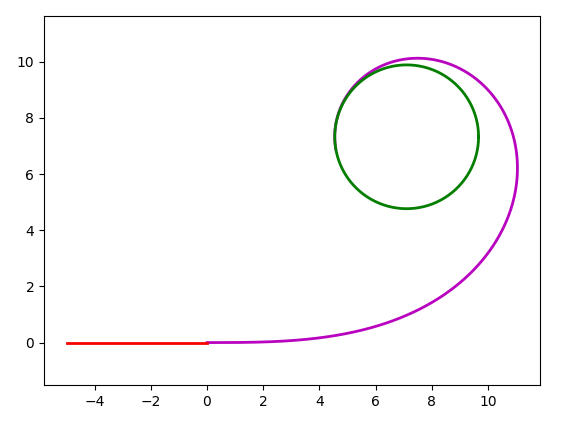
\includegraphics[width=0.4\linewidth]{img/clothoide2.jpg}
\end{center}

Het uiteindelijke doel van deze lesactiviteit is het kunnen aaneen koppelen van verschillende rechte wegen en rotonden door middel van gepaste clothoïden tot er een bruikbaar circuit ontstaat. Trek je hierbij niets aan van de verplichte rijrichting en van snijdingen van wegen.

\afbeelding[8.5cm]{img/uw clothoide.jpg}{}{}

\begin{tabular}{rr}
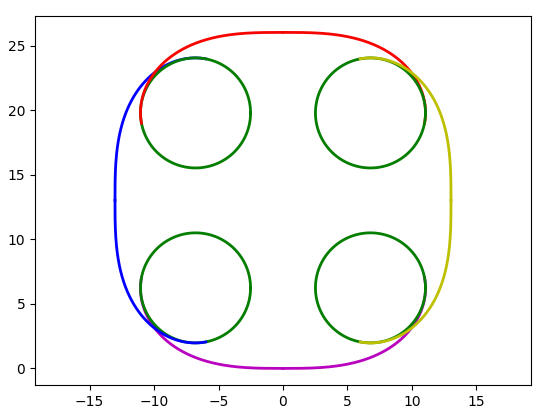
\includegraphics[scale=0.45]{img/clot10.jpg} & 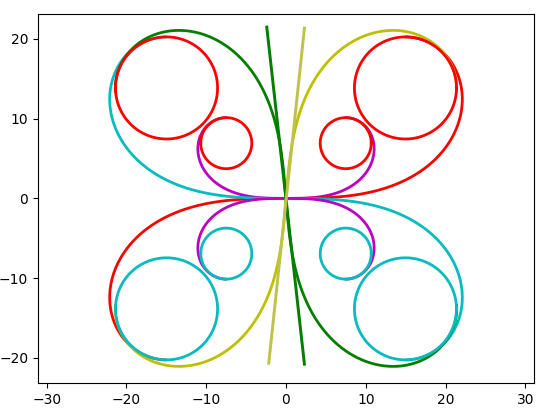
\includegraphics[scale=0.45]{img/vlinder2.jpg}\\
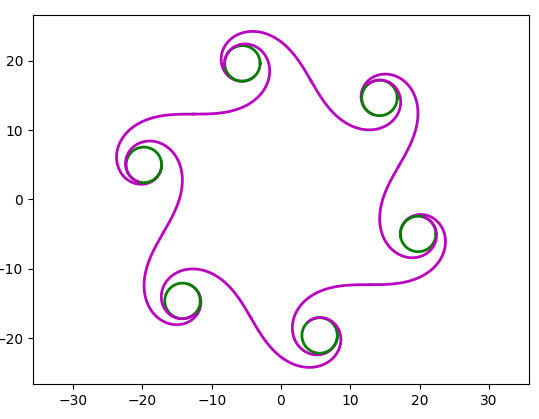
\includegraphics[scale=0.45]{img/clot12.jpg} & 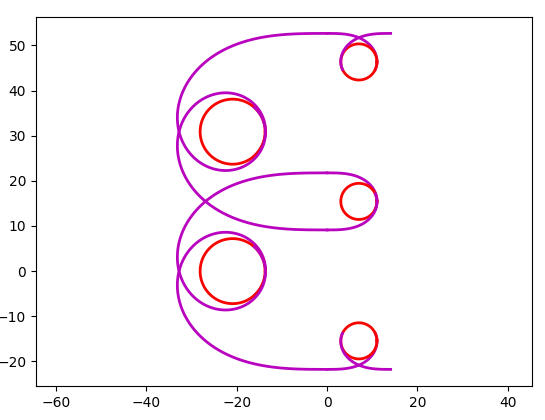
\includegraphics[scale=0.45]{img/clot14.jpg}
\end{tabular}


Open nu het programma Python en neem de volgende programmaregels over. Probeer aan de hand van de onderstaande vragen goed te begrijpen wat de functie is van elk van deze programmaregels. Laat het programma lopen en aanschouw de verschijning van een paarse clothoïdeboog.\\ 


\begin{kader}{Python}{Een verloopkromme tussen een rechte weg en een cirkelvormige rotonde}
1. \qquad  import matplotlib.pyplot as plt\\
2. \qquad import numpy as np\\
3. \\
4. \qquad \textcolor{red}{\# constanten en variabelen}\\
5. \qquad ds=.01\\
6. \qquad a=8\\
7. \qquad n=2000\\
8. \qquad x=0; xcoordinaten=[0]\\
9. \qquad y=0; ycoordinaten=[0]\\
10. \qquad s=0\\
11.\\
12. \qquad \textcolor{red}{\# de plot van een clothoide}\\
13. \qquad for i in range(n):\\
14. \qquad\qquad   s=s+ds\\
15. \qquad\qquad   alfa=s**2/(2*a**2)\\
16. \qquad\qquad   x=x+ds*np.cos(alfa); y=y+ds*np.sin(alfa)\\
17.  \qquad\qquad  xcoordinaten.append(x); ycoordinaten.append(y)\\
18. \qquad plt.plot(xcoordinaten, ycoordinaten, '-m', linewidth=2)\\
19.\\
20. \qquad \textcolor{red}{\# de plot van een lijnstuk}\\
21. \qquad..........\\
22. \\
23. \qquad \textcolor{red}{\# de plot van een cirkel}\\
24. \qquad..........\\
25. \\
26. \qquad \textcolor{red}{\# plotten van de grafieken}\\
27. \qquad plt.axis('equal')\\
28. \qquad plt.show()\\
\end{kader}

	\begin{vraagenantwoord}
		\vraag{In de eerste twee regels worden de gekende bibliotheekprogramma's matplotlib en numpy geladen. Waar worden ze verderop in het programma gebruikt?}
		\antwoord{Matplotlib wordt gebruikt bij het plotten. Je herkent de instructies uit Matplotlib aan het begin van hun naam: `plt'. Numpy wordt gebruikt bij numerieke operaties. Je herkent bijvoorbeeld: `np.cos' en `np.sin'.}
		
		\vraag{Hier en daar zie je een regel die met een hekje (\#) begint. Wat is de betekenis van dit hekje?}
		\antwoord{Regels met een hekje vooraan worden niet door de computer gelezen. Ze bevatten enkel informatie voor de programmeur en zijn medewerkers.}
		
		\vraag{In plaats van een vloeiende kromme te tekenen, tekenen we een aaneenschakeling van korte lijnstukjes met lengte d$s$. De eindpunten van deze lijnstukjes worden vanaf lijn 13 berekend. Vooraf leggen we alle constanten en beginwaarden van variabelen vast. Verklaar de regels 5 tot 10.}
		\antwoord{We tekenen een clothoïde waarvoor $a=8$. Er worden 2000 aaneensluitende lijnstukjes getekend met een lengte van 0,01 m. De clothoïde vertrekt uit het punt (0, 0). De x-coördinaten van de aansluitingspunten van de lijnstukken worden bewaard in de lijst \emph{xcoördinaten} en de y-coördinaten in de lijst \emph{ycoordinaten}. Aanvankelijk staan enkel de coördinaten van het vertrekpunt in deze lijsten. Bij de start is de afgelegde weg over de clothoïdeboog gelijk aan 0.}
		
		\vraag{Vanaf regel 13 tot en met 18 worden de deelpunten van de clothoïde berekend voor de opbouw van de grafiek. Verklaar deze regels.}
		\antwoord{De 4 inspringende instructies worden 2000 keer herhaald. Eerst wordt de afgelegde weg verhoogd met een lengte $ds$. Daarna wordt de richting van de raaklijn berekend met de formule (\ref{eindformule}). De machtsverheffing wordt in Python voorgesteld door een dubbel sterretje. In de volgende lijn worden de coördinaten van een nieuw deelpunt berekend uit die van zijn voorganger. We voegen deze nieuwe x-coördinaat en y-coördinaat achteraan toe aan de lijsten \emph{xcoördinaten} en \emph{ycoördinaten}. Als de lus 2000 keer doorlopen is, maken we een plot klaar met een lijndikte gelijk aan 2. Je kunt in tutorials op het internet opzoeken dat `-m' staat voor een ononderbroken lijn in magenta.}
		
		\vraag{Verklaar de laatste twee zinnetjes van het programma.}
		\antwoord{De voorlaatste instructie zorgt voor een gelijke ijking op de beide assen. Die hebben we straks zeker nodig. De ronde rotonde mag er immers niet uitzien als een ovale rotonde (een ovonde). De laatste zin zorgt er voor dat alle plots die in het programma berekend zijn, getekend worden. Momenteel is dit alleen nog maar een clothoïde.}
		
		\vraag{Welke instructie kun je ter hoogte van lijn 21 toevoegen om een rood lijnstuk te plotten van het punt $(-5, 0)$ tot $(0,0)$?}
		\antwoord{We gebruiken hiervoor de instructie: \emph{plt.plot([-5,0],[0,0],'-r',linewidth=2)}. Let op: in de eerste lijst staan de x-coördinaten van de twee eindpunten en in de tweede lijst staan de y-coördinaten van de eindpunten.}
		
		\vraag{Tot slot voegen we ter hoogte van lijn 24 de instructie toe om de gepaste cirkel  aan het krullende einde van de clothoïde vast te maken. Voor je hieraan begint, moet je twee vragen oplossen. Hoe bereken je de straal van deze cirkel? En hoe bereken je de coördinaten van het middelpunt?}
		\antwoord{De straal berekenen we met de formule: \emph{r=(a**2)/s}. Dit is een variatie op formule (\ref{booglengte}). Voor het middelpunt van de cirkel gebruiken we de instructies: \emph{xmid=x+r*np.cos(alfa+np.pi/2)} en \emph{ymid=y+r*np.sin(alfa+np.pi/2)}.}
		
		\vraag{Zoek in een Python-tutorial op hoe je een cirkel tekent met een gegeven middelpunt en een gegeven straal. Teken deze cirkel bij voorkeur aan de hand van de parametervergelijking van de cirkel.}

		\vraag{Maak nu zelf een compositie met meerdere rotonden en meerdere verloopkrommen en programmeer ze met Python. De rotonden mogen een gelijke of een verschillende straal hebben. De verloopkrommen mogen de omloopszin bewaren of omkeren. De techniek om deze compositie te maken, bestaat er telkens uit om één enkele rotonde te tekenen die je met een clothoïde met de negatieve $x$-as verbindt (met het aansluitingspunt in de oorsprong). Deze constructie moet je naar de gepaste plaats in het vlak schuiven, roteren en spiegelen. Heb je hulp nodig om deze transformaties wiskundig te vertalen, spreek je leerkracht dan aan.}

	\end{vraagenantwoord}
	
\end{lesactiviteit}




\stopcontents[inhoudloep]		% om inhoud voor het loep artikel te eindigen


%% BRONNEN %%%%%%%%%%%%%%%%%%%%%%%%%%%%%%%%%%%%%%%%%%%%%%%%%%%%%%%%%%%%%%%%%%%%%
\newpage

\begin{bronnen}
\item Aarts, J., Garst, S. (2017). \emph{Een verkenning van krommen. Nu met GeoGebra.} Zebrareeks deel 49. Amsterdam: Epsilon.

\item Correia de Sà (2008). Cinq courbes avec leur histoire: la quadratrice, la spirale, la conchoïde, la cissoïde et la cycloïde. \emph{History and Epistemology in Mathematics Education. Proceedings of the 5th European Summer University.} Pragues: Vydavatelský servis Pizen.

\item Ferréol, R. (2009). Oeuf de Hügelschäffer\url{https://mathcurve.com/courbes2d/oeuf/oeuf.shtml}

\item mAnasa-taraMgiNI (2021). The shape of dinosaure eggs. \url{https://manasataramgini.wordpress.com/2021/09/08/the-shape-of-dinosaur-eggs/}

\item Roelens, M. (1994). Christiaan Huygens als gastdocent. \emph{Uitwiskeling 10/1}, 19-62. (Paragraaf 4 gaat over het gebruik van cycloïden om het slingeruurwerk te verbeteren.)

\item Roelens, M. (1994b). Bespreking van [Treitz, K. (1993). Die Zykloide. \emph{Die mathematische und naturwissenschaftliche Unterricht 46/6}], \emph{Uitwiskeling 10/2}, 63-68. (Hoe Roberval raaklijnen aan de cycloïde construeert en de oppervlakte onder een cycloïdeboog berekent, en ook hoe de gebroeders Bernoulli bewijzen dat de cycloïde de `snelste glijbaan' is tussen twee punten.)

\item Roelens, M., Willems, J. (2005). Oppervlakte en volume door de eeuwen heen. \emph{Uitwiskeling 21/3}, 16-37. (Paragraaf 4 vertelt hoe Roberval de oppervlakte onder een cycloïdeboog berekent.)

\item Roelens, M. (2006). Bespreking van [Rolfs, J. (2005). Wie krumm ist die Banane? Krümmung und Kurven. \emph{Der Mathematikunterricht 51/4}], \emph{Uitwiskeling 22/2}.

\item Roelens, M. (2012). Weerkaatsing in een kop koffie. \emph{Uitwiskeling 28/4}, 6-9.

\item van de Craats, J., Mulder, H. (1989). Soepel door de bocht. \emph{Pythagoras 8/3}, 1-10.

\item Van den Broeck, L. (2011). Bespreking van [Bair, J., Henry, V. (2011). Sur le théorème de Mamikon. \emph{Losanges 12}], \emph{Uitwiskeling 27/4}, 49-54. (Met onder meer de berekening van de oppervlakte onder een cycloïdeboog op een andere manier.)

\end{bronnen}